\documentclass[a4paper, 12pt]{article}

% english
\usepackage[english]{babel}
\usepackage{lmodern}

% biblio
\usepackage{csquotes}
\usepackage[backend=biber, language=english]{biblatex}
\addbibresource{./biblio.bib}

% packages
\usepackage{fullpage}       % really narrow margins
\usepackage{graphicx}       % \includegraphics
\usepackage{amsmath}        % \text
\usepackage{multirow}       % \multirow   
\usepackage{enumitem}       % \setitemsize
\usepackage{appendix}       % appendix env
\usepackage{pgf, tikz}      % network architecture
\usetikzlibrary{positioning}

% center vertically
\usepackage{titling}        
\renewcommand\maketitlehooka{\null\mbox{}\vfill}
\renewcommand\maketitlehookd{\vfill\null}

% misc
\addto\captionsenglish{\def\chaptername{Part}}    % Part/Chapter
\renewcommand\thesection{\arabic{section}}        % arabic numbers
\setlength\parindent{0pt}                         % no indentation
\setitemize{itemsep=0em}                          % no space between itms

% code (default C++)
\usepackage{listings}
\usepackage{xcolor}
\definecolor{keyword}{rgb}{0.76,0.18,0.64}
\definecolor{directive}{rgb}{0.47,0.28,0.18}
\definecolor{string}{rgb}{0.85,0.16,0.14}
\definecolor{comment}{rgb}{0.43,0.65,0.38}
\lstdefinestyle{cpp}{
  language=C++,
  tabsize=2,
  keepspaces=true,
  showspaces=false,
  showtabs=false,
  showstringspaces=false,
  basicstyle=\ttfamily\footnotesize,
  keywordstyle=\color{keyword}\ttfamily,
  stringstyle=\color{string}\ttfamily,
  commentstyle=\color{comment}\ttfamily,
  morecomment=[l][\color{directive}]{\#}
}
\lstdefinestyle{xml}{
  language=C++,
  tabsize=2,
  keepspaces=true,
  showspaces=false,
  showtabs=false,
  showstringspaces=false,
  basicstyle=\ttfamily\footnotesize,
  stringstyle=\color{string},
  identifierstyle=\color{directive},
  keywordstyle=\color{directive},
  morestring=[b]",
  moredelim=[s]{>}{<},
  morecomment=[s]{<?}{?>},
  morekeywords={} % list attr here
}

\title{\textit{Hadoop} for Roboticists}
\author{Olivier Deiss\\
Supervised by Prof. C. Pradalier\\
UMI 2958 - GeorgiaTech Lorraine\\Metz, France}

\begin{document}

\begin{titlingpage}
\maketitle
\end{titlingpage}

\newpage
\tableofcontents
%\listoffigures
\newpage

\section{Introduction}

The objective of this tutorial is to give an overview of \textit{Hadoop}, its possibilities and its use in Robotics, as well as to provide explanations about the setup, design of mapreduce jobs and troubleshooting. \textit{Hadoop} is a powerful software: while this tutorial is enough to get an overview and a better understanding of the framework and how to use it, we won't be covering here all the possibilities that \textit{Hadoop} offers.

~\\
This tutorial is based on my experience while working on a Special Problem. I included all the information I have been looking for and everything I think can be useful when learning how to use \textit{Hadoop}. Finally, while reading this tutorial, be aware that I am far from being a \textit{Hadoop} expert and that I just started to learn about \textit{Hadoop}. This is just a summary of the best of my knowledge at the time of writing.

~\\
After presenting \textit{Hadoop} and how to set up a cluster, we will mainly focus on developing jobs in C++. Although jobs are usually written in Java, there are applications for which we need to be able to use C++. One of such situations is for being able to use the ROS API in our jobs. This will allow us to analyze datasets stored as \textit{rosbag}s as one possible application.

\section{About \textit{Hadoop}}

  \subsection{What is it?}

In short, Apache\textsuperscript{TM} \textit{Hadoop}\textsuperscript{\textregistered} is an open-source software framework for distributed storage and distributed processing of very large datasets on computer clusters built from commodity hardware. The true advantage of \textit{Hadoop} is how it handles scalability and insane amounts of unstructured data. \textit{Hadoop} works well on clusters of thousands of nodes. Here is a definition of the software from Apache's \textit{Hadoop} page:

\begin{quote}
It is designed to scale up from single servers to thousands of machines, each offering local computation and storage. Rather than rely on hardware to deliver high-availability, the library itself is designed to detect and handle failures at the application layer, so delivering a highly-available service on top of a cluster of computers, each of which may be prone to failures.
\end{quote}

\textit{Hadoop} is supported by Hortonworks and Cloudera. Facebook and Yahoo! have been the first companies to massively use \textit{Hadoop}; the software is now used by a majority of companies. Google's research papers \cite{google_1} \cite{google_2} inspired the \textit{Hadoop} File System and the \textit{MapReduce} implementation.

  \subsection{How does it work?}

Before jumping into the technical part of the tutorial, this section will introduce the main components of Hadoop as well as an overview of what is a job. We will also introduce the architecture of Hadoop clusters and what processes need to run on the machines.

    \subsubsection{Components}
  
\textit{Hadoop} is the union of \textit{base modules} and lots of other modules built on top of \textit{Hadoop}. We will only focus on the \textit{base modules} here. The base modules are the following ones:
\begin{itemize}
  \item \textit{\textit{Hadoop} Common}: this is a core module that provides libraries to the other modules.
  \item \textit{\textit{Hadoop} Distributed File System (HDFS)}: HDFS is a distributed file system on which we will be storing the data we want to analyze using \textit{Hadoop}. Alternatives to HDFS exist, but HDFS remains a good choice for the following reasons \cite{horton}: first the cost of storing data on HDFS is really low compared to other solutions that might not be open-source. HDFS is also tailored for MapReduce and allows a very high bandwidth even on very low-cost shared networks. Last, HDFS is designed to work on commodity hardware, and thus can handle failures and lost data autonomously.
  \item \textit{\textit{Hadoop} YARN}: YARN is used for the scheduling of the applications and the resource management.
  \item \textit{\textit{Hadoop} MapReduce}: \textit{MapReduce} is an implementation of the \textit{MapReduce} programming model. This is the framework we will use while writing jobs.
\end{itemize}

If you want to work with data, the first step is to upload it on HDFS. The next step is to write a \textit{MapReduce} job that will be later run on the cluster. The scheduling will be taken care of by YARN.

~\\
Among the other available auxiliary projects built on top of \textit{Hadoop}, Hive gives an SQL-like interface to run queries on the data stored on HDFS. Another one, HBase, is a distributed database based on Google's BigTable for storing large quantities of sparse data.

    \subsubsection{Writing jobs}

Jobs are the applications that are run on the data stored on HDFS. Actually, \textit{Hadoop} can also be run as a standalone application, without HDFS, but we won't be using \textit{Hadoop} this way. A simple application consists of two parts: a Mapper and a Reducer. The framework reads the input data and provides pairs \texttt{<key, value>} to the Mapper. By default, \textit{Hadoop} provides pairs with the following format: \texttt{<offset, line>}. Applications can provide their own Reader and Writers to customize these operations.

~\\
The Mapper receives these pairs and outputs another pair. This is all it does, and yet allows any kind of computation -- we will see examples later. The Mapper can put whatever information is useful in these pairs. The Reducer receives the pairs from the Mapper and outputs the final pairs \texttt{<key, value>} that will be the output of the job.

~\\
\textit{Hadoop} is written in Java and as a result, most of the documentation and online support is in Java. However, it is possible to write jobs in C++ using \textit{Hadoop} Pipes. This is what we will be doing since we are roboticists who want to be able to use the \textit{ROS} API in our jobs.

    \subsubsection{Cluster Architecture}

Hadoop runs on clusters of -- often thousands of -- computers. For huge datasets that span over multiple racks, HDFS provides location awareness: the processing happens on nodes that are close to the requested data: this reduces network traffic and is one of the key advantages of using HDFS. The setup we will describe here is a much smaller one, using a cluster one master node and five slave nodes.

~\\
A typical \textit{Hadoop} setup has the following structure:
\begin{itemize}
  \item \textit{Master} node: this node stores information about where is stored a specific information on the cluster. If this node becomes unavailable, the cluster as a whole becomes unavailable. For this reason, it is possible to run a second process on the same machine, which will handle the requests if the main process crashes.
  \item \textit{Slave} nodes: these nodes are the workers. They store the data and execute the jobs when requested.
\end{itemize}

In this tutorial, we will use the cluster as a model the cluster I have been using which has the following structure:

\begin{center}
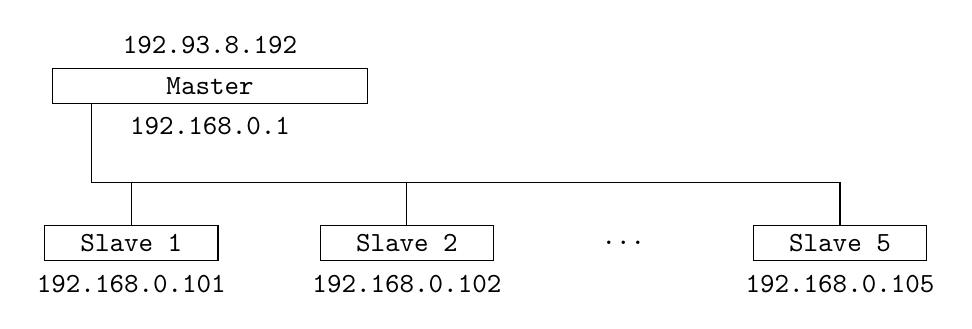
\begin{tikzpicture}
% machines
\node[minimum width=4cm, draw, rectangle] (M) at (0, 1) {\texttt{Master}};
\node[minimum width=2.2cm, draw, rectangle] (S1) at (-1, -1) {\texttt{Slave 1}};
\node[minimum width=2.2cm, draw, rectangle] (S2) at (2.5, -1) {\texttt{Slave 2}};
\node[minimum width=2.2cm, rectangle] (Sd) at (5.25, -1) {\texttt{...}};
\node[minimum width=2.2cm, draw, rectangle] (S5) at (8, -1) {\texttt{Slave 5}};
\node[below=0.05cm of S1] (IPS1) {\texttt{192.168.0.101}};
\node[below=0.05cm of S2] (IPS2) {\texttt{192.168.0.102}};
\node[below=0.05cm of S5] (IPS5) {\texttt{192.168.0.105}};
\node[above=0.05cm of M] (IPME) {\texttt{192.93.8.192}};
\node[below=0.05cm of M] (IPMI) {\texttt{192.168.0.1}};

\draw ([xshift=0.5cm]M.south west) |- + (0, -1) -| (S1);
\draw (S1.south) + (0, 1) -| (S2);
\draw (S2.south) + (0, 1) -| (S5);
\end{tikzpicture}
\end{center}

Here is a list of the processes that run on the nodes. Some processes are used for HDFS while the other category is used during the \textit{MapReduce} phase:
\begin{itemize}
  \item \textit{NameNode}, \textit{JobTracker}: these processes run on the Master node. The \textit{NameNode} is used as a registry of the data in the cluster, and the JobTracker is used during the \textit{MapReduce} phase. A \textit{SecondaryNameNode} can be run for the safety reasons discussed just above.
  \item \textit{DataNode}, \textit{TaskTracker}: these processes belong to the slaves. Note that it is also possible to run these processes on the Master node in small clusters. The \textit{DataNode} handles the storage and the \textit{TaskTracker} becomes useful during the \textit{MapReduce} phase.
\end{itemize}

\section{Setting Up a \textit{Hadoop} Cluster}

Now that we have scratched the surface of Hadoop in the previous introduction, we are ready for the first step in using Hadoop. Before writing jobs, we need to set up the structure on which we will launch these jobs. This step is about setting up a Hadoop cluster.

Hadoop can be run on one single node, and it might be useful to start from there to get familiar with the tools. The single node setup is well explained on the Apache tutorial \cite{hadoop_single_node_setup}. Here, we will directly go to the setup of a cluster of multiple nodes. We will then run the example mapreduce jobs, before we can start developing jobs in C++.

~\\
We will start by installing \textit{Hadoop} on all our machines and setting up all the tools that it needs. Then, we will configure our \textit{Hadoop} installation.

  \subsection{Installing \textit{Hadoop}}
  
Here, we will almost be following the Apache tutorial \cite{hadoop_single_node_setup}. The first step is to create a \textit{Hadoop} user: let's call it \textit{hadoop}, and everything \textit{Hadoop}-related we will do will be done with this user. I have been using \textit{Hadoop} 2.7.3 while working on this tutorial, you can get it here: http://hadoop.apache.org/releases.html. Install it wherever you find convenient, I chose \textit{/home/hadoop/bin}. We will also need to install Java if it is not already installed. \textit{Hadoop} 2.7 and later versions require Java 7 \cite{hadoop_java_versions}.

~\\
Assuming Java and \textit{Hadoop} are correctly installed, update your \textit{.bashrc} as follows, in order to give \textit{Hadoop} everything it needs to work properly. Here is what I have been using on my setup:

\begin{verbatim}
  export HADOOP_HOME=/home/hadoop/bin/hadoop-2.7.3
  export JAVA_HOME=/home/hadoop/bin/jdk1.8.0_102
  export PATH=${JAVA_HOME}/bin:${PATH}
  export HADOOP_CLASSPATH=${JAVA_HOME}/lib/tools.jar
\end{verbatim}

Note that \textit{HADOOP\_HOME} is not required, but it will make it easier for us to use this variable to refer to where \textit{Hadoop} is installed.  In the same file, I also decided to add \textit{bin} folders to my path. We will be using tools in \textit{HADOOP\_HOME/sbin}, which contains useful scripts, and in \textit{HADOOP\_HOME/bin}, which contains the hadoop and hdfs binaries:

\begin{verbatim}
  export PATH=${HADOOP_HOME}/sbin/:${HADOOP_HOME}/bin/:${PATH}
\end{verbatim}

We now jump to the configuration of \textit{Hadoop}. Four files, on each machine, need to be correctly updated. There is one file for each base module. The read-only versions, with the default values, have names \textit{base-module-default.xml}. The files that will need to be updated on the machines have the \textit{-site.xml} suffix instead. They are listed below:
\begin{itemize}
  \item \textit{HADOOP\_HOME/etc/hadoop/core-site.xml}: this file contains the core configuration. One important setting we will put in there is how to reach the file system.
  \item \textit{HADOOP\_HOME/etc/hadoop/hdfs-site.xml}: this is the configuration of the file system: the replication level, where to store the data, and the different types of nodes.
  \item \textit{HADOOP\_HOME/etc/hadoop/yarn-site.xml}: configuration for YARN, like how to reach the \textit{ResourceManager}.
  \item \textit{HADOOP\_HOME/etc/hadoop/mapred-site.xml}: this file contains the configuration for the \textit{MapReduce} jobs: they need to know how to reach the \textit{JobTracker.}
\end{itemize}

The entire configuration goes into these four files. The parameters will influence the way \textit{Hadoop} performs the tasks and you should have a look at the read-only versions of these files for a detailed explanation of the different parameters \cite{hadoop_core_default} \cite{hadoop_hdfs_default} \cite{hadoop_yarn_default} \cite{hadoop_mapred_default}.

~\\
Here I give the set of parameters that I have been using with my \textit{Hadoop} setup. This configuration works well for simple tasks but you will likely need to tune the parameters if you plan to make extensive use of \textit{Hadoop}.

    \subsubsection{Master Node}

The configuration differs from master and slave nodes. We will be listing here the minimum set of parameters that need to be set on the master node's configuration files. All we need to do is put the following \texttt{<property>} tags between the \texttt{<configuration>} and \texttt{</configuration>} tags:

\begin{itemize}
  \item \textit{core-site.xml}: here we will be telling hadoop how to reach the \textit{NameNode}. Since our \textit{NameNode} is the Master node, this parameter should link to the Master node:
    \begin{lstlisting}[style=xml]
      <property>
        <name>fs.defaultFS</name>
        <value>hdfs://192.93.8.197:9000</value>
      </property>
    \end{lstlisting}
  \item \textit{hdfs-site.xml}: in this file we can set the replication level and where to store the files on the machine. We choose a replication level of 3, note that this replication level should approximately be equal to the square root of the number of nodes in your cluster \cite{hadoop_mapred_default}:
    \begin{lstlisting}[style=xml]
      <property>
        <name>dfs.replication</name>
        <value>3</value>
      </property>
      <property>
        <name>dfs.namenode.name.dir</name>
        <value>file:///home/hadoop/hadoop_data/namenode</value>
      </property>
    \end{lstlisting}
  \item \textit{yarn-site.xml}: this is the configuration for YARN. Here, we tell YARN how to reach the \textit{ResourceManager}, and that we want to perform \textit{MapReduce} operations:
    \begin{lstlisting}[style=xml]
      <property>
        <name>yarn.nodemanager.aux-services</name>
        <value>mapreduce_shuffle</value>
      </property>
      <property>
        <name>yarn.resourcemanager.hostname</name>
        <value>192.93.8.197</value>
      </property>
    \end{lstlisting}
  \item \textit{mapred-site.xml}: last, we need to give the address of the \textit{JobTracker} to \textit{MapReduce,} and we can also set the replication level for the submitted jobs. By default, the value for \texttt{mapreduce.client.submit.file.replication} is set to 10, which will lead to under-replicated blocks in your setup if not changed.
    \begin{lstlisting}[style=xml]
      <property>
        <name>mapreduce.jobtracker.address<name>
        <value>192.93.8.197:54311</value>
      </property>
      <property>
        <name>mapreduce.client.submit.file.replication</name>
        <value>2<value>
      </property>
    \end{lstlisting}
\end{itemize}

    \subsubsection{Slave Nodes}

Now let's see the configuration of the slave nodes. Here again we need to configure the four files listed above, but the configuration is exactly the same for \textit{core-site.xml} and \textit{yarn-site.xml}.
    
\begin{itemize}
  \item \textit{hdfs-site.xml}: the configuration of HDFS will now require us to specify where to store the data, hence we will be using the property \texttt{dfs.datanode.data.dir} instead of \texttt{dfs.namenode.name.dir}:
    \begin{lstlisting}[style=xml]
      <property>
        <name>dfs.replication</name>
        <value>3</value>
      </property>
      <property>
        <name>dfs.datanode.data.dir</name>
        <value>file:///home/hadoop/hadoop_data/datanode</value>
      </property>
    \end{lstlisting}
  \item \textit{mapred-site.xml}: in this file we will be adding one more property compared to the configuration for the Master node, in order to tell the worker nodes to use YARN as their \textit{MapReduce} framework:
    \begin{lstlisting}[style=xml]
      <property>
        <name>mapreduce.jobtracker.address<name>
        <value>192.93.8.197:54311</value>
      </property>
      <property>
        <name>mapreduce.client.submit.file.replication</name>
        <value>2<value>
      </property>
      <property>
        <name>mapreduce.framework.name</name>
        <value>yarn<value>
      </property>
    \end{lstlisting}
\end{itemize}
    
  \subsection{Hostnames, \textit{SSH}}

Now Hadoop should be correctly configured. But before we can start the nodes, we need to setup \textit{ssh} on all the machines and set the hostnames of each as well. This is really important, and can be the source of lots of errors if not set right at first. \textit{Hadoop} communicates over \textit{ssh} between different nodes. It also uses the machines hostnames rather than their IP addresses.

~\\
Therefore we need to set up these two things. First, let's get \textit{ssh} working. \textit{Hadoop} requires that each node can reach any other node over \textit{ssh}, without a passphrase \cite{hadoop_single_node_setup}. If you cannot do so, running the following commands should solve the issue:

\begin{verbatim}
  $ ssh-keygen -t dsa -P '' -f /home/hadoop/.ssh/id_dsa
  $ cat /home/hadoop/.ssh/id_dsa.pub >> /home/hadoop/.ssh/authorized_keys
  $ chmod 0600 /home/hadoop/.ssh/authorized_keys
\end{verbatim}

If \textit{ssh} is correctly configured, we can set the hostnames of our machines. On each machine, we need to update \textit{/etc/hosts} as well as \textit{/etc/hostname}.

    \subsubsection{Slave Nodes}
    
On the Slave nodes, let's start by setting the hostname of each machine. On my setup, I have the hostnames \texttt{slave1} to \texttt{slave5}. In the \textit{/etc/hosts} file, each worker node should have access to all the other nodes. Each of my slave nodes has the following file:

\begin{verbatim}
  127.0.0.1       localhost
  192.168.0.101   slave1
  192.168.0.102   slave2
  192.168.0.103   slave3
  192.168.0.104   slave4
  192.168.0.105   slave5
  192.168.0.1     cluster3
\end{verbatim}

    \subsubsection{Master Node}
    
On the Master node, we will need to have a list of all the available workers, in addition to correctly setting up the files \textit{/etc/hostname} and \textit{/etc/hosts}. The hostname of my master node is \texttt{cluster3}, and its \textit{hosts} file looks like the following:

\begin{verbatim}
  128.0.0.1       localhost localhost
  127.0.1.1       cluster3.domain.fr cluster3
  192.168.0.101   slave1 slave1
  192.168.0.102   slave2 slave2
  192.168.0.103   slave3 slave3
  192.168.0.104   slave4 slave4
  192.168.0.105   slave5 slave5
\end{verbatim}

As stated above, we will also need to indicate what machines are available as masters or slaves in the \textit{Hadoop} configuration. This is done in the files \textit{masters} and \textit{slaves} in \textit{HADOOP\_HOME/etc/hadoop}. If these files don't exist on your setup, just create them with this name.

~\\
For \textit{HADOOP\_HOME/etc/hadoop/masters}, we only have one master node so the file has just one entry:

\begin{verbatim}
  cluster3
\end{verbatim}

For \textit{HADOOP\_HOME/etc/hadoop/slaves}, I have listed the hostnames of the five available worker nodes:

\begin{verbatim}
  slave1
  slave2
  slave3
  slave4
  slave5
\end{verbatim}

  \subsection{Starting the Cluster}
  
Everything should now be correctly set up and we should be able to run the cluster. We first need to format the file system:

\begin{verbatim}
  $ hdfs namenode -format
\end{verbatim}

Now that the file system is formatted, we can create our home folder where we will later upload our input files:

\begin{verbatim}
  $ hdfs dfs -mkdir -p /user/hadoop
\end{verbatim}

Note that a lot of basic commands are available on HDFS. We have just used \texttt{mkdir}, but likewise, \texttt{ls}, \texttt{cat}, \texttt{mv} are also available. We can now start HDFS, then YARN. The scripts are located in \textit{HADOOP\_HOME/sbin}:

\begin{verbatim}
  HADOOP_HOME $ sbin/start-dfs.sh
  HADOOP_HOME $ sbin/start-yarn.sh
\end{verbatim}

If you have added this folder to your \texttt{PATH}, you should be able to run them without specifying the folder. Alternatively, you can run \texttt{start-all.sh}, which works well and starts both at once, even though it is deprecated. If you run \texttt{jps}, you should see this list on the master node:
\begin{verbatim}
  NameNode
  SecondaryNameNode
  ResourceManager
\end{verbatim}

If you run the same command on one of the slaves, you should see this list instead:
\begin{verbatim}
  DataNode
  NodeManager
\end{verbatim}

Anytime, you can go to http://IP:50070 -- with the IP address of the master node -- to see the nodes usage in real-time. You can monitor all the applications at http://IP:8088. Useful tools are also available in command line:

\begin{verbatim}
  $ hdfs dfsadmin -printTopology   # displays a topology of the setup
  $ hdfs dfsadmin -report          # creates a complete report
\end{verbatim}

  \subsection{\textit{MapReduce} Example}

To make sure our cluster is correctly set up, let's try to run a first \textit{MapReduce} job. A job is provided in the \textit{Hadoop} installation. It just counts the words in the input files and displays them with the associated count. 

~\\
To run this example we first need to create our input. An input is a folder containing files we want to work on. You can just copy all the \textit{xml} files in \textit{HADOOP\_HOME/etc/hadoop} in a folder \textit{input}, and upload this folder on HDFS:

\begin{verbatim}
  HADOOP_HOME $ mkdir input
  HADOOP_HOME $ cp etc/hadoop/*.xml input
  HADOOP_HOME $ hdfs dfs -put input .
\end{verbatim}

You can make sure the folder has been correctly uploaded by running \texttt{hdfs dfs -ls}. We are now ready to launch the job:

\begin{verbatim}
  $ hadoop jar \
           share/hadoop/mapreduce/hadoop-mapreduce-examples-2.7.3.jar \
           grep input output 'dfs[a-z.]+'
\end{verbatim}

This command tells \textit{Hadoop} to launch a jar, located in \textit{HADOOP\_HOME/share/...}. In this jar, we are interested in launching the class \texttt{grep} -- not the command-line grep tool -- to perform the job. \textit{Hadoop} will use \textit{input} as its input folder and will output the results in \textit{output}. Finally, the results will contain all the words that match the regular expression \texttt{dfs[a-z.]+}.

~\\
After a few seconds, the job should -- successfully -- complete. If the job failed, maybe you can find some help in the troubleshooting section at the end of this tutorial. You can also check the GUI anytime to check if everything is working properly. The output is available in \textit{output}. We can read it from the file system, or download it and then read it:

\begin{verbatim}
  $ hdfs dfs -cat output/*                        # read from HDFS
  $ hdfs dfs -get output output && cat output/*   # download then read
\end{verbatim}

If everything worked as expected, we are ready to go to the next step, where we will be using both \textit{ROS} and \textit{Hadoop Pipes} in a C++ mapreduce job. You can find more information about writing jobs in Java, and tutorials on the Apache website \cite{hadoop_mapreduce_tutorial}.

\section{Writing Jobs in C++ using \textit{Hadoop Pipes}}

We now have a working installation of \textit{Hadoop}, but we can only work with Java. Our goal is to be able to write jobs in C++, combining \textit{ROS} and \textit{Hadoop} in the same job. \textit{Hadoop} provides \textit{Hadoop Pipes}, which allows us to write jobs in C++. We will first see how to get \textit{Hadoop Pipes} working, and then we will need to work a bit more to get \textit{Hadoop Pipes} and \textit{ROS} working together.

  \subsection{Running a \textit{Hadoop Pipes} job}
  
    \subsubsection{Compiling and Launching the Job}

We will start with a simple example, following \cite{smith_pipes}. The code we are going to use in our first example is available in appendix \ref{wordcount}. We will need a Makefile in order to compile this program. This one will work, assuming you are on a 64-bit version:

\begin{verbatim}
  CC             = g++
  HADOOP_INSTALL = /home/hadoop/bin/hadoop-2.7.3
  CPPFLAGS       = -m64 -std=c++00x -I$(HADOOP_INSTALL)/include
  LIBS           = -L$(HADOOP_INSTALL)/lib -lhadooppipes -lhadoop
                   -lhadooputils -lcrypto -lpthread -lssl

  word_count: word_count.cpp
    $(CC) $(CPPFLAGS) $< -o $@ -Wall $(LIBS) -g -O2
\end{verbatim}

You might need to install additional packages like \texttt{libssl-dev} to be able to link without errors. Compile using \texttt{make word\_count}. If you are getting errors, make sure you have correctly set \texttt{HADOOP\_INSTALL} and that all the libraries are installed.

~\\
If you managed to compile the program, we will first need to upload it on the file system before we can run it:

\begin{verbatim}
  $ hdfs dfs -put word_count .
\end{verbatim}

Assuming you still have the input folder from the previous example, we can now run the job. If you did not previously delete the old output folder, you will get an error. To delete the old \textit{output} folder:

\begin{verbatim}
  $ hdfs dfs -rm -r -f output
\end{verbatim}

We can now run the job:

\begin{verbatim}
  $ hadoop pipes -D hadoop.pipes.java.recordreader=true \
                 -D hadoop.pipes.java.recordwriter=true \
                 -input input -output output \
                 -program word_count
\end{verbatim}

The first two options tell \textit{Hadoop} to use the default Java \textit{RecordReader} and \textit{RecordWriter} classes. It is possible to implement these classes to get a custom behavior, but I could not find much documentation about this. There exists an example, \textit{wordcount-nopipe.cc}, in appendix \ref{wordcountnopipe}, which shows how to do that. Be aware that this only works with local file reads though.

~\\
If everything ran successfully, we can print the output:

\begin{verbatim}
  $ hdfs dfs -cat output/*
\end{verbatim}

    \subsubsection{How Does This Job Work?}
  
Let's quickly go through the code of this job and see what it does. This simple \textit{MapReduce} job has two classes: a \textit{Mapper} and a \textit{Reducer}. Pretty straightforward.

~\\
Let's first focus on the \textit{Mapper}. Its constructor takes one parameter, \texttt{context} that we are not using here. The interesting part is the \texttt{map} function, which takes a \texttt{MapContext} as its only parameter. This object contains all the pairs provided to this mapper from one partition of the input. The key and values are accessible via \texttt{getInputKey()} and \texttt{getInputValue()} respectively. For each word, the \textit{Mapper} outputs a pair \texttt{<word, 1>}. Note that everything needs to be a string. This is all that it does.

~\\
We can now study the \texttt{Reducer}. The reduce function is called with a context that contains all the pairs with the same key. In order to count the words, we therefore need to initialize a counter to 0 and increment it for each pair in the context. This is done in the \texttt{while} loop. After what we can simply output a pair with the same key as the input key, and the value of the counter as the output value. If you wonder why we emitted ones in the \textit{Mapper}, yes, this was absolutely useless, but we still needed to output some values.

~\\
This really is how this job works. If you want to familiarize yourself with the \textit{MapReduce} framework, you can find lots of examples of jobs online. Even though they are in Java, it is a good start to get an intuition of how jobs should be written. You can follow the Apache tutorial on \textit{MapReduce} \cite{hadoop_mapreduce_tutorial}, or this great tutorial \cite{slideshare_tuto}.

~\\
So we managed to get \textit{Hadoop Pipes} working and we -- almost -- wrote our first job. In the next section, we will see how to use \textit{Hadoop Pipes} and \textit{ROS} for writing our jobs.

  \subsection{Using \textit{Hadoop Pipes} with \textit{ROS}}

We finally get to the section that initiated the writing of this tutorial: how to use \textit{Hadoop} to write jobs that use ROS. \textit{Hadoop} and Java are great for lots of domains, and jobs should be written in Java if possible. Using Pipes should only be used when there is no alternative. The fact that we want to use ROS in our jobs is one great reason to do so. The following will help you understand how to write jobs using the C++ \textit{ROS} API. If you do not want to use \textit{ROS}, you can skip this section.

    \subsubsection{Creating New Libraries}

Unfortunately, the provided \textit{Hadoop} libraries don't work well with the \textit{ROS} libraries. This is related to the compiler Application Binary Interface (ABI). \textit{ROS} and the \textit{Hadoop} library don't use the same ABI, hence they work poorly together. 

~\\
To get them working, you will need to recompile \textit{Hadoop} from source. After downloading, following the steps on the Apache guide \cite{native_libs}, run the following commands:

\begin{verbatim}
  mvn package -Pdist,native -DskipTests -Dtar
\end{verbatim}

In order to compile \textit{Hadoop} successfully, you will need to install \texttt{protoc} -- Protocol Buffers -- version 2.5.0 and this version only. You can get it on Google's github \cite{google_github}. The archive should be available at: https://github.com/google/protobuf/archive/v2.5.0.tar.gz.

~\\
You will get the newly-bilt library in \textit{hadoop-dist/target/hadoop-2.7.3/lib/native}. From now on, use these libraries instead of the ones in \textit{HADOOP\_HOME/lib} and everything should work fine.

    \subsubsection{A Job with \textit{ROS} and \textit{Hadoop Pipes}}
  
We can now go back to our initial goal of compiling a job with \textit{Hadoop Pipes} that makes use of the \textit{ROS} API. We will first see how to update our Makefile, them we will show how to use Catkin to do all the work for us.

~\\
We will need to update our Makefile to link the \textit{ROS} libraries. Note that I've put the newly-built libraries in \textit{/home/hadoop/lib/hadoop/lib}.

\begin{verbatim}
  CC             = g++
  HADOOP_INSTALL = /home/hadoop/bin/hadoop-2.7.3
  CPPFLAGS       = -m64 -std=c++00x -I$(HADOOP_INSTALL)/include
                   -I/opt/ros/kinetic/include
  LIBS           = -L/home/hadoop/lib/hadoop/lib -lhadooppipes -lhadoop
                   -lhadooputils -lcrypto -lpthread -lssl
                   -L/opt/ros/kinetic/lib -lroscpp -lrosconsole -lrostime
                   -lrosbag -lrosbag_storage

  ros_example: ros_example.cpp
    $(CC) $(CPPFLAGS) $< -o $@ -Wall $(LIBS) -g -O2
\end{verbatim}

This new Makefile indicates where to find the right \textit{libraries}. This is all we needed to add. Using this, you should be able to compile jobs in C++, using \textit{Hadoop} and \textit{ROS} libraries.

    \subsubsection{Using \textit{Hadoop}, \textit{ROS} and \textit{Catkin}}

For modern versions of ROS, compilation is made using \textit{Catkin}. In order to keep using it to compile our jobs, we just need to create a package with the right dependencies and \textit{CMakeLists.txt} file. Let's follow the procedure from the beginning: first we need to create a new package:

\begin{verbatim}
  $ catkin_create_pkg ros_example
\end{verbatim}

We then need to edit the file \textit{package.xml}. In the dependencies section, add \texttt{roscpp} to specify that we will be using C++, as well as all the other needed dependencies for your project:

\begin{lstlisting}[style=xml]
  <buildtool_depend>catkin</buildtool_depend>
  <build_depend>roscpp</build_depend>
  <build_depend>rostime</build_depend>
  <build_depend>rosbag</build_depend>
  <build_depend>rosbag_storage</build_depend>
  <build_depend>rosconsole</build_depend>
  <build_depend>std_msgs</build_depend>
  <run_depend>roscpp</run_depend>
  <run_depend>rostime</run_depend>
  <run_depend>rosbag</run_depend>
  <run_depend>rosbag_storage</run_depend>
  <run_depend>rosconsole</run_depend>
  <run_depend>std_msgs</run_depend>
\end{lstlisting}

More important, we need to edit the \textit{CMakeLists.txt} file to include \textit{Pipes} and link \textit{Hadoop} as well as \textit{ROS}:

\begin{lstlisting}[style=xml]
  cmake_minimum_required(VERSION 2.8.3)
  project(example)
  find_package(catkin REQUIRED COMPONENTS
    roscpp rosconsole rostime rosbag rosbag_storage
  )
  catkin_package(
    CATKIN_DEPENDS roscpp
  )
  include_directories(~/bin/hadoop-2.7.3/include ${catkin_INCLUDE_DIRS})
  add_definitions(-g -ggdb -std=c++14 -Wall -O3)
  link_directories(/home/hadoop/lib/hadoop/lib)
  add_executable(example ros_example.cpp)
  target_link_libraries(example
    hadooppipes hadoop hadooputils crypto pthread ssl
  )
  target_link_libraries(example ${catkin_LIBRARIES})
  install(TARGETS example
    ARCHIVE DESTINATION ${CATKIN_PACKAGE_LIB_DESTINATION}
    LIBRARY DESTINATION ${CATKIN_PACKAGE_LIB_DESTINATION}
    RUNTIME DESTINATION ${CATKIN_PACKAGE_BIN_DESTINATION}
  )
\end{lstlisting}

There is nothing really special about this file. It is a standard \textit{CMakeLists.txt} file with instructions to include and link everything required by \textit{Hadoop}.

~\\
With this file, we should be able to compile our code using \texttt{catkin\_make}. The binary will be in the directory \texttt{build} of your \textit{Catkin} workspace.

  \subsection{An Example of Job to Analyze rosbags}

To complete our introduction on using ROS with \textit{Hadoop} we are going to write a job that analyzes rosbags and counts the different values for a given topic in the file.

~\\
The structure is very similar to that of the first job we have studied. We will have one class for the \textit{Mapper}, one for the \textit{Reducer}. This does not change. What changes is that rosbags cannot be read directly by \textit{Hadoop}. While looking for a more elegant solution, we are going to store our rosbags on a shared folder that will be accessed by the nodes through NFS. The job's input will instead be a folder containing the paths of these files. Therefore each entry of the \textit{Map} task will be the path of a file that we can open using the \textit{ROS} API.

~\\
Once the file is open, we need to create a view of this file for the topic of our choice. The view can provide us with iterators through the file. As for the word count, we now just need to iterate through the values and output them as the key, with a value that will not be used. After iterating through the values, we close the bag and return.

~\\
Now for the \textit{Reducer}, we read all the values, and increment a counter for every value. After iterating through all the keys, we output the key and its counter.

~\\
The code for this example is available in appendix \ref{valuecount}. You can compile it with the command \texttt{catkin\_make}, upload the program on HDFS and run it with an input being a folder of files containing paths to your actual rosbags

\section{Troubleshooting}

Before even being able to write this simple tutorial, I have come a long way and had to face and solve lots of issues. I tried to list them all here with ways to solve them. They were mostly due to configuration problems so you might not have as many errors as I did. Otherwise this section is the right one.

  \subsection{Starting \textit{Hadoop}}

    \subsubsection*{All the processes did not start}
    
After running \texttt{start-all.sh} or \texttt{start-dfs.sh} and \texttt{start-yarn.sh}, you should always check with \texttt{jps} if all the processes started successfully. If they did not, you will find why in the logs. Most likely, you've been trying to restart them too quickly and the ports are reserved. You can check what process is using your port with:

\begin{verbatim}
  sudo netstat -ap | grep :50090
\end{verbatim}

Then kill this process and try again.

    \subsubsection*{Hadoop does not work after a restart}
    
Make sure you have correctly set the folders for \textit{Hadoop} in \textit{core-site.xml} on all the machines. By default, \textit{Hadoop} writes in \textit{/tmp}.

  \subsection{MapReduce}

Let's start with issues when launching a job. First you should go have a look in the log files. They are in \textit{HADOOP\_HOME/logs/user} and will always tell you the source of the error. Alternatively, you can check if everything is ok from a configuration aspect with:

\begin{verbatim}
  $ hdfs dfsadmin -report
\end{verbatim}
  
    \subsubsection*{Running a Job Fails}

Hadoop will not overwrite an output folder. You should always make sure to delete the previous output folders or to specify a different folder for later jobs. If \textit{Hadoop} is trying to reach a node and is having trouble, check if all the nodes are up. Sometimes some nodes are \textit{decommissioned} and you need to start the right processes again. Running \texttt{start-all.sh} from the master should launch all the missing nodes.

~\\
Once again, checking the logs will most likely tell you the source of the error. Another error related to the use of ROS is that some nodes could be missing libraries required by your job. You need to make sure all your nodes are correctly configured before going on.
   
    \subsubsection*{The job hangs at \textit{map 0\%, reduce 0\%}}

Make sure you have set the hostnames right, and that you can \textit{ssh} to any node without a passphrase. In any case, the logs should tell you what happened, but this issue happened to me due to network issues. This can also be due to an error in your code that causes an exception. Typically, if your \textit{Mapper} is correct but your \textit{Reducer} is wrong, you will most likely see the task hang at \textit{map 100\%, reduce 0\%}.
    
  \subsection{Monitoring}
  
    \subsubsection*{Positive amount of under-replicated blocks}
    
You need to check if your settings for replication are correctly set. Also, make sure \texttt{mapreduce.client.submit.file.replication} is set, otherwise its default value of 10 will lead to under-replicated blocks if your cluster has less than ten machines.

  \subsection{Writing Jobs}

Finally, while writing jobs, make sure to never cut a stream, meaning that a \textit{Mapper} or \textit{Reducer} should only return once it has extracted all the pairs that it was given. Also, make sure your stream has pairs available to be read before extracting one.

\section{Conclusion}

In this tutorial, we have seen how to set up a cluster for \textit{Hadoop}. We have also studied how to compile jobs for \textit{Hadoop} in C++, using \textit{Hadoop Pipes}, and how to use \textit{ROS} for our jobs.

~\\
Regarding performances, during my work I have managed to interpolate three days of data in 40 minutes, using the cluster described above in the tutorial.  However the way I have been using \textit{Hadoop}, through shared files on NFS, would not scale properly to larger structures where we could not benefit of the rack-awareness. Instead, with a preprocessing step to extract the data in the \textit{rosbags} in \textit{csv} files, we should be able to use Hadoop the way it is supposed to be used.

~\\
I hope you managed to set up your own cluster and that this document has been helpful. Now that your \textit{Hadoop} is working, it's time to write jobs!

\newpage
\begin{appendices}
%\addtocontents{toc}{\setcounter{tocdepth}{-1}}

  \section{WordCount.cpp}
  \label{wordcount} 

\begin{lstlisting}[style=cpp]
#include <algorithm>
#include <limits>
#include <string>

#include "stdint.h"

#include "hadoop/Pipes.hh"
#include "hadoop/TemplateFactory.hh"
#include "hadoop/StringUtils.hh"

class WordCountMapper : public HadoopPipes::Mapper {
  public:
  WordCountMapper(HadoopPipes::TaskContext& context) {}
  // map function: receives a line, outputs (word,"1") to reducer.
  void map(HadoopPipes::MapContext& context) {
    // get line of text
    std::string line = context.getInputValue();
    // split it into words
    std::vector<string> words = HadoopUtils::splitString(line, " ");
    // emit each word tuple (word, "1")
    for (unsigned int i=0 ; i < words.size() ; i++) {
      context.emit(words[i], HadoopUtils::toString(1));
    }
  }
};

class WordCountReducer : public HadoopPipes::Reducer {
  public:
  WordCountReducer(HadoopPipes::TaskContext& context) {}
  void reduce(HadoopPipes::ReduceContext& context) {
    int count = 0;
    // get all tuples with the same key, and count their numbers
    while (context.nextValue()) {
      count += HadoopUtils::toInt(context.getInputValue());
    }
    // emit (word, count)
    context.emit(context.getInputKey(), HadoopUtils::toString(count));
  }
};

int main(int argc, char *argv[]) {
  return HadoopPipes::runTask(
    HadoopPipes::TemplateFactory<WordCountMapper,
                                  WordCountReducer>()
  );
} 
\end{lstlisting}

  \newpage
  \section{WordCount-NoPipe.cc}
  \label{wordcountnopipe}

\begin{lstlisting}[style=cpp]
/**
  * Licensed to the Apache Software Foundation (ASF) under one
  * or more contributor license agreements.  See the NOTICE file
  * distributed with this work for additional information
  * regarding copyright ownership.  The ASF licenses this file
  * to you under the Apache License, Version 2.0 (the
  * "License"); you may not use this file except in compliance
  * with the License.  You may obtain a copy of the License at
  *
  *     http://www.apache.org/licenses/LICENSE-2.0
  *
  * Unless required by applicable law or agreed to in writing, software
  * distributed under the License is distributed on an "AS IS" BASIS,
  * WITHOUT WARRANTIES OR CONDITIONS OF ANY KIND, either express or
  * implied. See the License for the specific language governing
  * permissions and limitations under the License.
  */

#include "hadoop/Pipes.hh"
#include "hadoop/TemplateFactory.hh"
#include "hadoop/StringUtils.hh"
#include "hadoop/SerialUtils.hh"

#include <stdio.h>
#include <sys/types.h>
#include <sys/stat.h>

const std::string WORDCOUNT = "WORDCOUNT";
const std::string INPUT_WORDS = "INPUT_WORDS";
const std::string OUTPUT_WORDS = "OUTPUT_WORDS";

class WordCountMap: public HadoopPipes::Mapper {
  public:
  HadoopPipes::TaskContext::Counter* inputWords;

  WordCountMap(HadoopPipes::TaskContext& context) {
    inputWords = context.getCounter(WORDCOUNT, INPUT_WORDS);
  }

  void map(HadoopPipes::MapContext& context) {
    std::vector<std::string> words = 
      HadoopUtils::splitString(context.getInputValue(), " ");
    for (unsigned int i=0 ; i < words.size() ; i++) {
      context.emit(words[i], "1");
    }
    context.incrementCounter(inputWords, words.size());
  }
};

class WordCountReduce: public HadoopPipes::Reducer {
  public:
  HadoopPipes::TaskContext::Counter* outputWords;

  WordCountReduce(HadoopPipes::TaskContext& context) {
    outputWords = context.getCounter(WORDCOUNT, OUTPUT_WORDS);
  }

  void reduce(HadoopPipes::ReduceContext& context) {
    int sum = 0;
    while (context.nextValue()) {
      sum += HadoopUtils::toInt(context.getInputValue());
    }
    context.emit(context.getInputKey(), HadoopUtils::toString(sum));
    context.incrementCounter(outputWords, 1); 
  }
};

class WordCountReader: public HadoopPipes::RecordReader {
  private:
  int64_t bytesTotal;
  int64_t bytesRead;
  FILE* file;
  public:
  WordCountReader(HadoopPipes::MapContext& context) {
    std::string filename;
    HadoopUtils::StringInStream stream(context.getInputSplit());
    HadoopUtils::deserializeString(filename, stream);
    struct stat statResult;
    stat(filename.c_str(), &statResult);
    bytesTotal = statResult.st_size;
    bytesRead = 0;
    file = fopen(filename.c_str(), "rt");
    HADOOP_ASSERT(file != NULL, "failed to open " + filename);
  }

  ~WordCountReader() {
    fclose(file);
  }

  virtual bool next(std::string& key, std::string& value) {
    key = HadoopUtils::toString(ftell(file));
    int ch = getc(file);
    bytesRead += 1;
    value.clear();
    while (ch != -1 && ch != '\n') {
      value += ch;
      ch = getc(file);
      bytesRead += 1;
    }
    return ch != -1;
  }

  /**
    * The progress of the record reader through the split
    * as a value between 0.0 and 1.0.
    */
  virtual float getProgress() {
    if (bytesTotal > 0) {
      return (float)bytesRead / bytesTotal;
    } else {
      return 1.0f;
    }
  }
};

class WordCountWriter: public HadoopPipes::RecordWriter {
  private:
  FILE* file;
  public:
  WordCountWriter(HadoopPipes::ReduceContext& context) {
    const HadoopPipes::JobConf* job = context.getJobConf();
    int part = job->getInt("mapred.task.partition");
    std::string outDir = job->get("mapred.work.output.dir");
    // remove the file: schema substring
    std::string::size_type posn = outDir.find(":");
    HADOOP_ASSERT(posn != std::string::npos, 
                  "no schema found in output dir: " + outDir);
    outDir.erase(0, posn+1);
    mkdir(outDir.c_str(), 0777);
    std::string outFile = outDir + "/part-" +
                          HadoopUtils::toString(part);
    file = fopen(outFile.c_str(), "wt");
    HADOOP_ASSERT(file != NULL, "can't open file: " + outFile);
  }

  ~WordCountWriter() {
    fclose(file);
  }

  void emit(const std::string& key, const std::string& value) {
    fprintf(file, "%s -> %s\n", key.c_str(), value.c_str());
  }
};

int main(int argc, char *argv[]) {
  return HadoopPipes::runTask(
    HadoopPipes::TemplateFactory<WordCountMap, WordCountReduce,
                                  void, void, WordCountReader,
                                  WordCountWriter>()
  );
}
\end{lstlisting}

  \newpage
  \section{ros\_example.cpp}
  \label{valuecount}

\begin{lstlisting}[style=cpp]
#include <vector>

#include "Pipes.hh"
#include "StringUtils.hh"
#include "SerialUtils.hh"

#include "ros/ros.h"
#include "rosbag/view.h"
#include "rosbag/structures.h"
#include "geometry_msgs/Twist.h"

class ExampleMap : public HadoopPipes::Mapper {
 public:
  ExampleMap(HadoopPipes::TaskContext& context) {}
  void map(HadoopPipes::MapContext& context) {
    // extract paths from input
    std::vector<std::string> paths = 
        HadoopUtils::splitString(context.getInputValue(), " ");
    for (unsigned int i=0; i < paths.size(); ++i) {
      // open rosbag file, create a view and an iterator on this view
      std::string path = "/mnt/nfs/" + paths[i];
      rosbag::Bag bag(path);
      rosbag::View topic_view(bag, rosbag::TopicQuery("/cmd_vel"));
      rosbag::View::iterator j = topic_view.begin();
      // iterate through the values
      for (; j != topic_view.end(); j++) {
        // instantiate a message from the view
        boost::shared_ptr<geometry_msgs::Twist> m =
            j->instantiate<geometry_msgs::Twist>();
        // emit linear.x as a key, with random value
        context.emit("angular x " + std::to_string(m->angular.x), "1");
      }
      bag.close();
    }
  }
};

class ExampleReduce : public HadoopPipes::Reducer {
 public:
  ExampleReduce(HadoopPipes::TaskContext& context) {}
  void reduce(HadoopPipes::ReduceContext& context) {
    int count = 0;
    while (context.nextValue()) count++;
    // output the final result
    context.emit(context.getInputKey(), std::to_string(count));
  }
};

int main(int argc, char *argv[]) {
  return HadoopPipes::runTask(
    HadoopPipes::TemplateFactory<ExampleMap, ExampleReduce>()
  );
}
\end{lstlisting}

\end{appendices}

\newpage
\addcontentsline{toc}{section}{References}
\printbibliography

\end{document}


